\section{Motorcontoller}
The purpose of the Motorcontroller is to adjust the speed of the vehicle. In this design it is done by a PWM-signal and a MOSFET. It is of the utmost importance that the hardware affects the motor in the least possible way and thereby affecting the efficiency of the motor itself.

Aside from controlling the motor, this circuitry also senses the voltage and current consumption of the motor. This data is going to the PSoC and is here analyzed. There is, amongst other things, an overcurrent protection built in, to secure the PCB. For more information on this subject see \vref{sec:measurements}.

\subsection{Design}
There are several design considerations to take into account when designing this motorcontroller. The primary and most important feature to this design is the MOSFET that is used. Furthermore the resistor placed between the driver and the MOSFET, decides the amount of current going into the MOSFET and by that how fast it switches(more on this later). On figure \vref{fig:Motorcontroller} it is dubbed 'R18'. 

The figure below(\vref{fig:Motorcontroller}) shows a snippet of the motorcontroller. The parts left out are the measurements as discussed in \vref{sec:measurements}.

There are three components at use here:

\begin{itemize}
	\item{IRFB7530 = Power MOSFET}
	\item{MBR20200CT = Power Diode}
	\item{MCP1407 = MOSFET Driver}
\end{itemize}

The design considerations when using these specific components will be discussed here. Furthermore the components specific application purpose will be mentioned. Lastly, it will be explained as to why this component was chosen.  

\textbf{IRFB7530} \cite{IRFB7530}\\
When using a MOSFET to control a DC-motor, there are numerous precautions that must be taken into account. Most of the precautions will be mentioned further down, when designing the MOSFET driver. 

The MOSFET is the most wide-spread and reckoned way to control a DC-motor and therefore it is chosen here as well. Since the car is not required to run in reverse, it is implemented as a single component and not a H-bridge. This eases the implementation greatly.

This specific component is chosen as it consist of a very low on resistance and thereby the power dissipated in the component will be lower than for a similar MOSFET with a higher on resistance. The maximum on resistance, as described by the datasheet is mere 2 m$\Omega$. Due to a lower power dissipation the heatshink reqiured by the MOSFET to keep it within its operating range, can be smaller or even obsolete. When choosing a MOSFET with a low on resistance, as this is the case, it will come with a very high input capacitance. This is caused by the manufactoring proces of a MOSFET and the values are inversely proportional with each other. For this reason also it has been chosen to implement a MOSFET driver. 

The chosen MOSFET is overdimensioned for this purpose, as it can both endure a much higher current and voltage, than what the motor will operate at. This is done, as the stress that it will be put under during the race will be great and a breakdown would be more or less catastrophic. The specifications can be seen on the table in figure \vref{fig:MOSFET}.

The chosen MOSFET is in the TO-200 housing. This housing is chosen, so that if it is needed to mount the MOSFET on a heat sink it can be done conveniently.  

\begin{figure}[H]
	\centering
	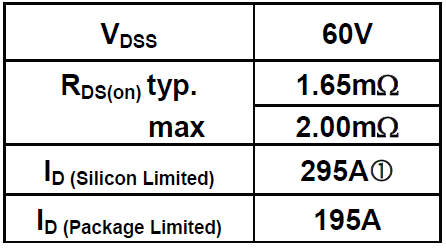
\includegraphics[width=0.85\linewidth]{Hardware/Pictures/MOSFET}
	\caption{MOSFET specifications}
	\label{fig:MOSFET}
\end{figure}

\textbf{MBR20200CT} \cite{MBR20200}

This diode is a flyback diode, in place to secure a known passage for the generated current by the motor, when the MOSFET is shut off. When the motor is supplied is supplied with a current it works as a motor, but when the current is shut off, the motor works as a generator. It is necessary to secure components from possible breaking down after trying to sink the current from the generated motor. The diode is placed in parallel with the motor.

A schottkey diode is chosen for its very fast switching time and less for the low voltage drop. This means that there is a smaller power dissipation in the diode and thereby less loss which equals a higher efficiency. 

This diode is chosen for its specifications to be able to withstand the current coming from the motor. It can be switched with another diode with similar specifications.

\textbf{MCP1407} \cite{MCP1407}

When using a MOSFET driver the design must live up to requirements set forth by the datasheet. This mostly consists of proper placement on the PCB layout, but also includes which capacitors to use as decoupling. But it also leaves a lot for the designer to choose, as there is no suggestions for connections. 

The decoupling capacitors are needed as there is high current requirements for driving the gate capacitance of a standard MOSFET and the IC is therefore in need of a local storage. This also means that the placement of the capacitors must be physically close to the IC to avoid stray capacitances. The capacitors chosen to perform the task, are the same as specified in the datasheet, 1 ceramic and 1 low ESR film capacitor. 

There is connected a resistor to the output pin of the driver. This is included for two reasons. The primary reason being that when using a MOSFET to drive an inductive load, as it is the case here, the di/dt must be reduced as to secure proper switching in the MOSFET. The second reason is to protect the MOSFET, more specific, the gate insultation, which could be damaged by the spikes caused by having an inductive load.

Increasing this resistors value would mean a slower switching time, but would be able to provide a more stable output and decrease ringing. The ringing is caused by the gate being in series with, albeit involuntarily, a small inductor caused by the PCB trace. By decreasing the value of the resistor the turn on peaks of the drain pin increases as well as the ringing. But it also increases the switching time, which makes it a trade off, and causes it to be a major point of optimization in the system. The only boundary for the resistor is that it must be of a certain value to ensure that the components in use doesn't go up in flames.   

The main reason for the choosing to use a driver for the MOSFET is that the PSoC only can deliver so much current. And since faster switching times, means less power loss in the MOSFET which is favorable for when designing a energy efficient vehicle. The argument could be made that the driver also consumes current, but the maximum current drawn from the driver at any time is 150 $\mu $A for typical values. With those numbers the benefits are set to outway the costs.  

This component was chosen as it was already implemented in the Rolling road design and therefore the group had both experience and spare parts of this. This component is easily interchangeable with other components of the same specifications. 

\begin{figure}[H]
	\centering
	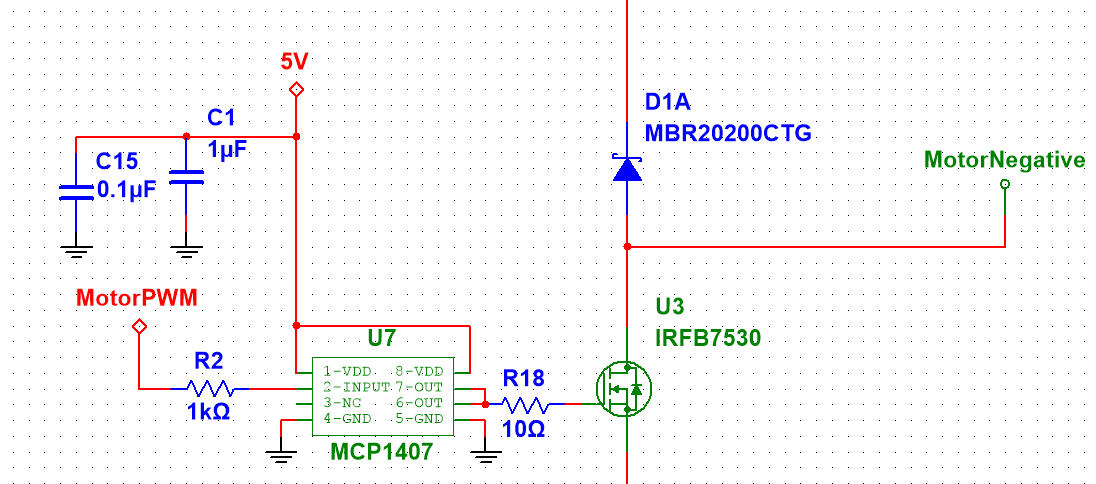
\includegraphics[width=0.85\linewidth]{Hardware/Pictures/Motorstyring}
	\caption{Motor controller hardware}
	\label{fig:Motorcontroller}
\end{figure}


\subsection{Unity test}
There is going to be conducted 2 tests for this module. The first test is a unity test that will make sure the general purpose of the circuitry is working as designed. The other test that will be conducted on this module is a stress test, that will simulate an entire run as it will be in London. 

Neither of these tests have been made at hand in, but are fairly straight forward to conduct. 

The first test consist of hooking up the motor and placing a PWM on the input of the MOSFET driver. Also there must be 48V connected and a working distribution block must be available. A succesful test here is composed of a motor that is rotating. 

The second test must contain the same start parameters as the previous test. The difference here is that this test must first of all run at least 45 minutes. This time should be sufficient to ensure that the testing is done for a long enough period that it can safely be stated that the MOSFET and surrounding circuit can withstand the power dissipation. To take the stress test even further it can programmed to run a higher speed or with a higher load. 